\documentclass{article}
\usepackage[utf8]{inputenc}
\usepackage{listings}
\usepackage{float}
\usepackage{graphicx}
\usepackage{fullpage}
\usepackage{caption}
\usepackage{subcaption}

%\renewcommand{\thesubsection}{\arabic{subsection}}
\renewcommand{\thesubsubsection}{\alph{subsubsection}}

\title{Pattern Recognition practical 1}
\author{Maikel Withagen (s1867733) \and Steven Bosch (s1861948)}
\date{September 2015}
\lstset{frame=single, numbers=left,language=Matlab}

\begin{document}

\maketitle

\section{Assignment 1}
\subsection{}
To compute the pair-wise correlation coefficients we used the following command:
\begin{lstlisting}[title= Input]
load('lab1_1.mat')
corrcoef(lab1_1)
\end{lstlisting}
This yields us the following table of correlation coefficients:
%\begin{lstlisting}[title= Output]
%   1.0000   -0.0615    0.7156
%  -0.0615    1.0000    0.5142
%   0.7156    0.5142    1.0000
%\end{lstlisting}
\begin{table}[H]
	\caption{\textit{Pair-wise correlation coefficients}}
	\vspace{0.1cm}
	\centering
	\begin{tabular}{|c|c|c|c|}
		\hline
		& Length & Age & Weight \\
		\hline
		Length & 1 & -0.0615 & 0.7156 \\
		\hline
		Age & -0.615 & 1 & 0.5142 \\
		\hline
		Weight & 0.7156 & 0.5142 & 1 \\ 
		\hline
	\end{tabular}
	\label{tab1.2}
\end{table}

\subsection{}

\begin{figure}[H]
	\centering

	\begin{subfigure}[b]{.45\linewidth}
		The two features for which the correlation is the largest are the first and third column, respectively the height and the weight.
		\centering
		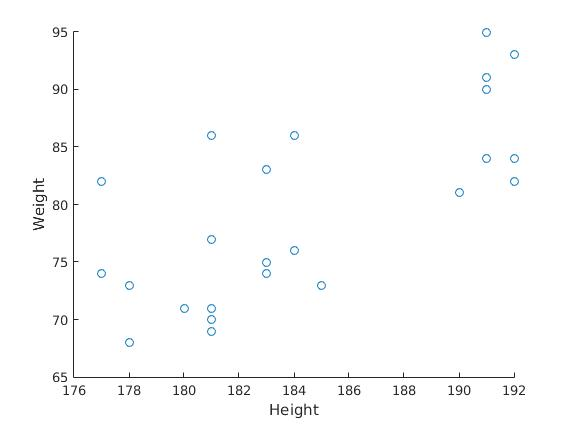
\includegraphics[width=\columnwidth]{plot_1_3_a.jpg}
		\caption{Scatterplot of weight to length}
		\label{fig1.3a}
	\end{subfigure}%
	\quad
	\begin{subfigure}[b]{.45\linewidth}
		The two features for which the correlation is the second largest are the second and third column, respectively the height and the weight.
		\centering
		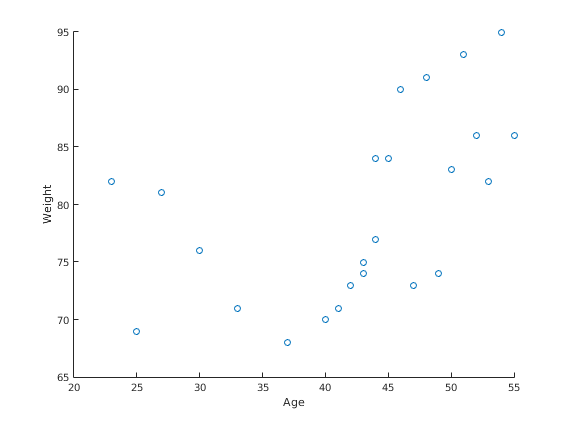
\includegraphics[width=\linewidth]{plot_1_3_b.png}
		\caption{Scatterplot of weight to age.}
		\label{fig1.3b}
	\end{subfigure}
	\caption{}
\end{figure}
From a scatterplot alone it is hard to draw conclusions about any possible relationships between the different features. 
We do get indications though; figure \ref{fig1.3a} shows that there is likely to be a correlation between the weight and the height.
An increase in weight seems to correspond to a (somewhat linear) increase in height. 
A similar kind of relationship can be seen in figure \ref{fig1.3b}, between the factors weight and age.

\section{Assignment 2}
\subsection{}
The following subsections show the code we used to acquire the 1000 Hamming distances for set S and D.
\subsubsection{}
To compute the set S we first create the set and fill it with zeros (line 1). Then for every element in the set we randomly pick a person and two random rows within that person and consequently load the actual content of these rows (lines 2-9). Then we compute the hamming distance between those two rows and store it within the appropriate place in the set (line 11). Finally the whole set is scaled so that every element in the set reflects the hamming distance between two elements instead of two rows.
\begin{lstlisting}[title = Code for set S]
hd_s = zeros(1,1000);
for i = 1:1000
  person = randi([1,20]);
  row1 = randi([1,20]);
  row2 = row1;
  while(row1 == row2)
    row2 = randi([1,20]);
  end
  load(sprintf('person%02d.mat',person));

  hd_s(i) = sum(abs(iriscode(row1,:)-iriscode(row2,:)));
end
hd_s = hd_s/30;
\end{lstlisting}
\subsubsection{}
To compute the set D we do the same thing except for the fact that we compute the hamming distances between rows of two different persons:
\begin{lstlisting}[title = Code for set D]
hd_d = zeros(1,1000);
for i = 1:1000
  person1 = randi([1,20]);
  row1 = randi([1,20]);
  row2 = randi([1,20]);
  person2 = person1;
  while(person1 == person2)
    person2 = randi([1,20]);
  end
  load(sprintf('person%02d.mat',person1));
  x = iriscode(row1,:);
  load(sprintf('person%02d.mat',person2));
  y = iriscode(row2,:);
  hd_d(i) = sum(abs(x-y));
end
hd_d = hd_d/30;
\end{lstlisting}

\subsection{}
\begin{figure}[H]
	\centering
	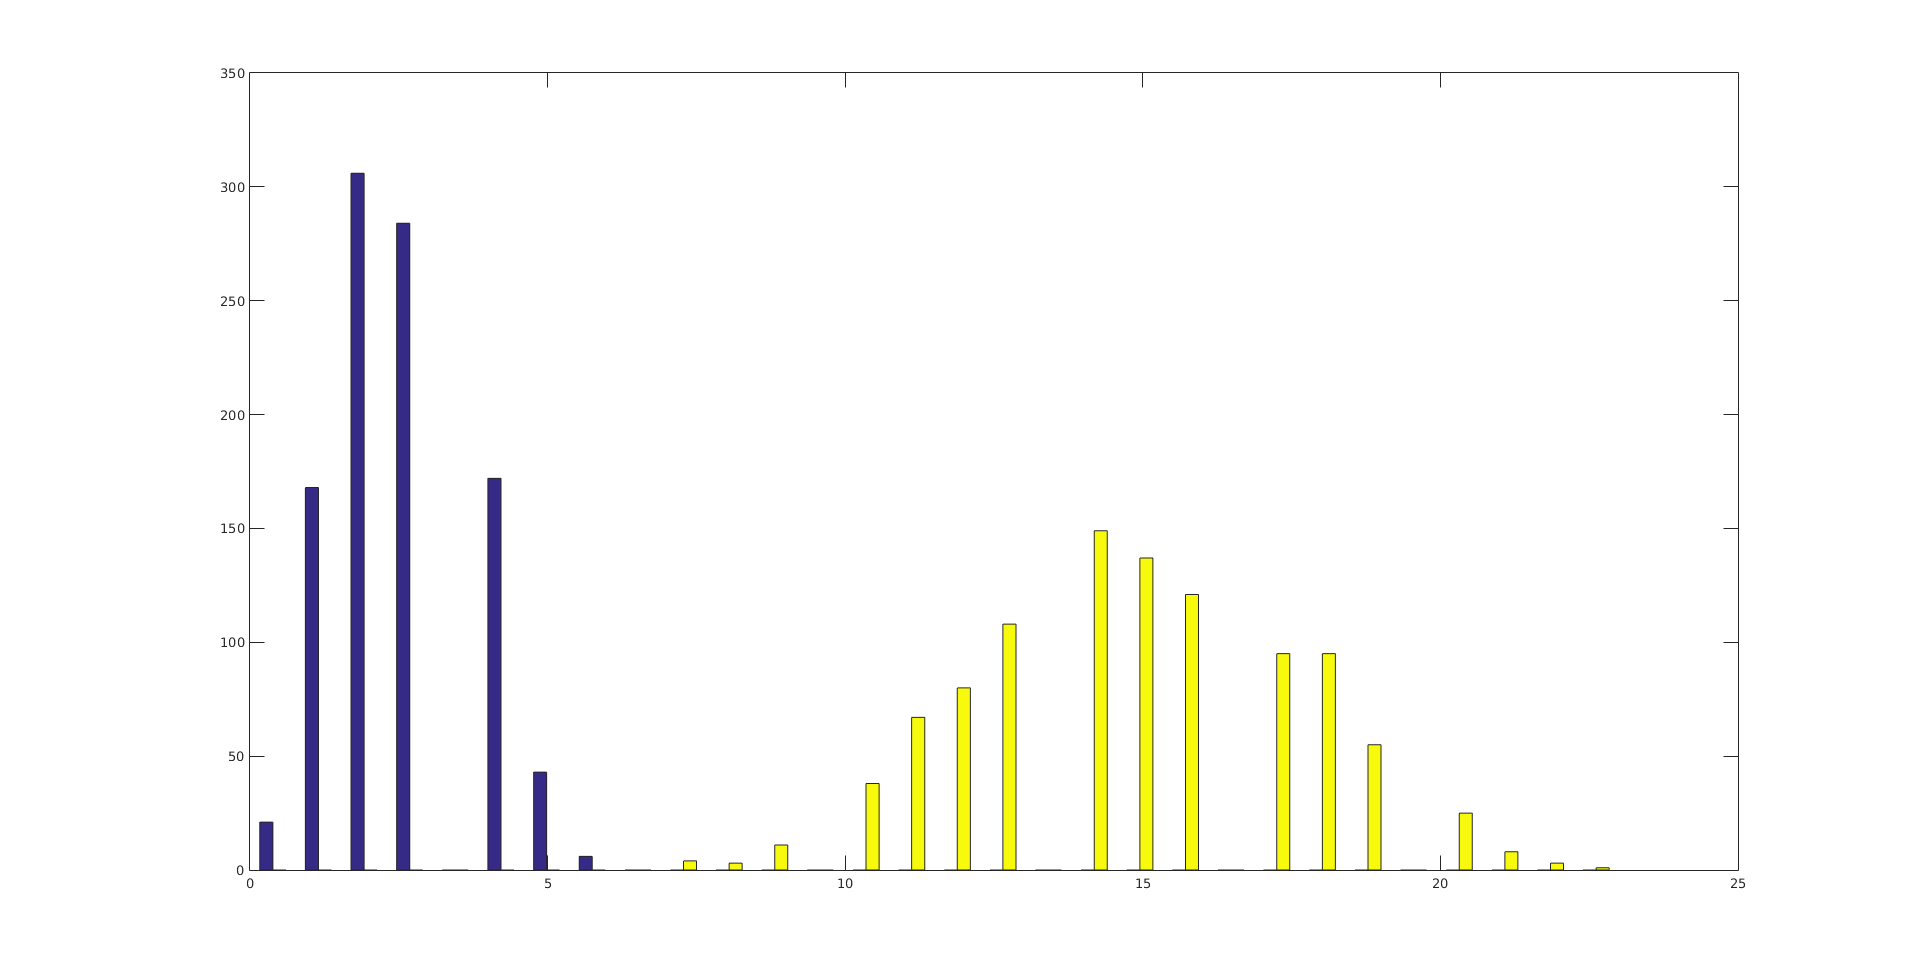
\includegraphics[width=.7\linewidth]{plot2_4.png}
	\caption{Histogram of sets S and D.}
	\label{fig2.4}
\end{figure}
Figure \ref{fig2.4} shows the histogram of sets S and D. The figure shows that the two distributions overlap very little, most of it around $hd = 5,6$.

\subsection{}
The means and variances of both of the sets are the following:
\begin{table}[H]
 \begin{tabular}{|c|c|c|c|}
  \hline
  Set & Mean & Variance & Standard deviation \\
  \hline
  S & 0.0825 & 0.0016 & 0.0398 \\
  \hline
  D & 0.4946 & 0.0079 & 0.0886 \\
  \hline
 \end{tabular}
 \caption{Means and variances of both of the sets}
 \label{tab2.5}
\end{table}
\noindent The prior propability of two bits being the same between persons the following is: $1-0.4946=0.5054$.
Using the formula $n=p(1-p)/\sigma^2$ we get $n=(0.4946*(1-0.4946))/(0.0886^2)\approx 31.84$ statistically independent bits that are needed to encode an iris pattern. This means that the current number of bits in the iris vectors is insufficient.

\subsection{}
We acquired the graph in figure \ref{fig2.6} (see the appendix for the matlab code we used).

\begin{figure}[H]
	\centering
	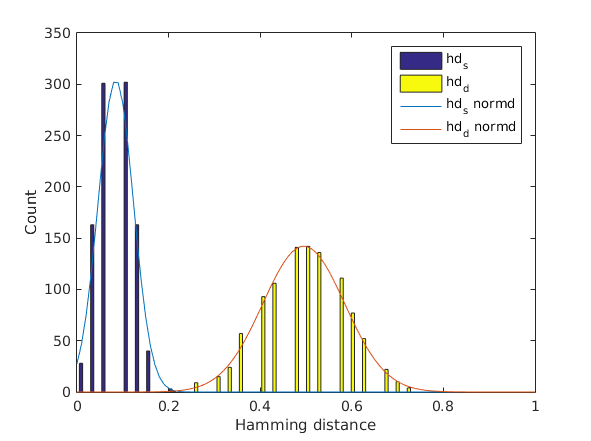
\includegraphics[width=.7\linewidth]{2_6.png}
	\caption{The histograms of sets S and D plotted with two Gaussian functions using the mean and variances.}
	\label{fig2.6}
\end{figure}
Figure \ref{fig2.6} shows the plot of the combined histograms and gaussian functions (note that the plot is slightly different from the previous subsections, because we reran the script in Matlab). The scaling is done by dividing the maximum value of the D and S sets by the maximum value of the initial Gaussian functions. This way the maximum value of the new Gaussian functions is the same as the maximum value of the D and S sets, so that the the Gaussians are nicely scaled to the histograms.

\subsection{}
\subsubsection{}
To estimate the value of the decision criterion we used the following code:
\begin{lstlisting}
% Calculate the cumulative distribution function for the 
% given x-value (range 0.000 - 1.000, with stepsize 0.001)
normc = normcdf([0:0.001:1],mean(hd_d),std(hd_d));
% Count the amount of x-values below the threshold value, minus 1 to correct 
% from starting from 0.000, and divide by 1000 to get the decision criterion
d = (sum(normc(:) <= 0.0005)-1)/1000;
\end{lstlisting}
This yielded the value 0.185 as criterion. This means that below a hamming distance of 0.185, we will erroneously classify two irisses as being from the same person.

\subsection{}
Using the criterion of 0.185, we get a false rejection rate of 0.0072, using the following code:
\begin{lstlisting}
% Same as before, now for set S
normc = normcdf([0:0.001:1],mean(hd_s),std(hd_s));
% False rejection is integral of HD > d is 1 - normc(d)
1 - normc((d*1000)+1)
\end{lstlisting}
This means that up to 0.72\% is falsely classified as being from two different persons.

\section{Assignment 3}
\subsection{Background}
The topic of biometric identification has been receiving a lot of attention lately. % Mooie opening xD
The use of fingerprints, facial features, and iris recognition are considered appropriate for identification.
Of these three, fingerprints and iris recognition are considered to be more accurate than facial features,
while facial featuresare more flexible, e.g.\ for the use in surveillance scenarios.
A possible improvement for the performance of facial feature identification is the combination of information from multiple sources,
for instance the ear.
Ear images can be obtained in a similar maner to face images, 
and a recent study suggests that they are comparable in recognition power\cite{chang2003comparison},
and a combination of the sources gives a significant improvement over their individual performance.
\subsection{Method}
\subsection{Achieved Results}
\subsection{Conclusion}

\bibliographystyle{plain}
\bibliography{cite}

\section*{Appendix}
Code for assignment 2.4:
\begin{lstlisting}
hold off;

% Making the histogram
hd = [hd_s;hd_d].'
hist(hd,30); xlabel('Hamming distance'), ylabel('Count');
hold on;

% Create scaled Gaussian plots
x2 = sum(hd_s(:) == mode(hd_s));
normd = normpdf([0:0.01:1],mean(hd_s),std(hd_s));
plot([0:0.01:1],normd*(x2/max(normd)));

x1 = sum(hd_d(:) == mode(hd_d));
normd = normpdf([0:0.01:1],mean(hd_d),std(hd_d));
plot([0:0.01:1],normd*(x1/max(normd)));

legend('hd_s', 'hd_d', 'hd_s normd', 'hd_d normd');
\end{lstlisting}
\end{document}
